%Créé par Claudine Allen en collaboration avec Jean-Raphaël Carrier
%Dernière modification JRC: 13 janvier 2014
%Élimination du labo de résistivité des matériaux (IV) à la fin de l'ère JRC + regroupement des labos VI & VII en début de pandémie COVID-19 => renumérotation IX -> VII maintenant
%Dernière modification CA: 4 novembre 2020
%Dernière modification JG:
%***ToDo***
% - préparer un signal de bruit pour montrer comment on se rapproche de sinus/cosinus avec Q qui augmente dans un filtre passe-bande,

\RequirePackage[l2tabu, orthodox]{nag} %Check for obsolete commands
\documentclass[canadien,12pt,oneside,letterpaper]{article}
%
%-----------------------------------------------------
%Loading packages
%
\usepackage[utf8]{inputenc}
\usepackage[T1]{fontenc}
\usepackage[canadien]{babel}
\usepackage{lmodern}
\usepackage{textcomp}
\usepackage{amsmath,amssymb}
\usepackage{siunitx}
\usepackage{xcolor}
\usepackage{hyperref}
\usepackage[all]{hypcap}
\usepackage{graphicx}
\usepackage[oldvoltagedirection,americanvoltages,americancurrents,siunitx]{circuitikz}
\usetikzlibrary{babel}
\usepackage{caption}
\usepackage{subcaption}
%\usepackage{subfig}
\usepackage[letterpaper,headheight=15pt]{geometry}
\usepackage{fancyhdr}
\usepackage{setspace}
%
%----------------------------------------------------
%Other configurations and layout
%
\sisetup{separate-uncertainty}
\captionsetup{font=small,labelfont=bf,margin=0.1\textwidth}
\pagestyle{fancy}
\fancyhf{}
\lhead{\textsl{GPH-2006/PHY-2002~---~Laboratoire~VII}}
\rhead{\textsl{Page \thepage}}
\setcounter{secnumdepth}{0}
\setlength{\parskip}{1.5ex plus0.5ex minus0.2ex}
%\onehalfspacing
\interfootnotelinepenalty=10000 %To avoid footnotes spreading on several pages.
%
%---------------------------------------------------
%
\title{\textbf{Atelier VII}\\Filtres passifs \& actifs\thanks{Auteurs: Claudine Allen, Jean-Raphaël Carrier, Jérémie Guilbert, Daniel Côté}}
\renewcommand\footnotemark{}
\date{}


\begin{document}

\maketitle \vspace{-2cm}

\section{Objectifs}

Il est très fréquent qu'un signal d'intérêt doit être filtré pour atténuer les effets d'un bruit quelconque (haute fréquence par exemple) ou une lente dérive d'un signal soit-disant constant (basse fréquence). Vous avez vu les filtres RC pour faire des filtres passe-bas ou passe-haut.  Vous travaillerez donc avec les concepts de filtres RC, de résistance (impédance) d'entrée et de sortie, de réponses en fréquences que vous approfondirez tout au long de l'atelier. Dans cet atelier, vous devrez:
\begin{enumerate}
\item concevoir un filtre RC approprié pour une source donnée, 
\item le fabriquer, 
\item le connecter correctement,
\item et valider son bon fonctionnement dans les conditions décrites. 
\end{enumerate}
 
%Une fonction essentielle accomplie par des circuits électriques dans le travail expérimental est celle de filtrer un signal. On peut alors retirer des fréquences indésirables et généralement obtenir une mesure plus fidèle avec un meilleur rapport signal sur bruit, par exemple. L’effet de différents filtres sur le gain et la phase de signaux en tension sera donc étudié dans ce laboratoire à l’aide du diagramme de Bode. En particulier, les performances de différents design de filtres avec des composants uniquement passifs seront comparées à un design intégrant un amplificateur opérationnel actif. Ce laboratoire, en association avec le deuxième devoir, a aussi pour objectif d’approfondir la compréhension de l’étudiant.e des domaines temporel et fréquentiel dans le cadre des transformations de Laplace et Fourier. La relation entre délai temporel et déphasage sera donc examinée pour le filtre RC. 
%Dans l'approche pédagogique de préparation et conception de ce laboratoire, l'étudiant.e développera progressivement une méthodologie de travail plus autonome en transition vers la pratique d'une profession de recherche en sciences et génie.
%
%Sous-objectif: observer et quantifier le délai temporel du signal en tension aux bornes des différents composants de ce circuit RC série.
%
% \textbf{Sous-objectif} : démontrer que ce même circuit RC série agit en filtre passe-haut ou passe-bas en prenant les mesures appropriées pour construire les diagrammes de Bode du gain ET de la phase en fonction de la fréquence.
%
% \textbf{Sous-objectif} : démontrer, à l'aide des diagrammes de Bode, qu'un circuit RLC série agit en filtre passe-bande dont le facteur de qualité $Q$ varie avec d'autres valeurs de $R, L$ et $C$.
%
% \textbf{Sous-objectif} : examiner comment les filtres (a) RC série de premier ordre, (b) RC de troisième ordre, (c) Butterworth en topologie Cauer de troisième ordre et (d) Butterworth en topologie Sallen-Key de troisième ordre, vont dévier du comportement idéal d'un filtre passe-bas, c'est-à-dire une fonction échelon de Heaviside centrée sur la fréquence de coupure. 

%Les travaux effectués aborderont les objectifs d’ensemble 1, 2, 4, 5, 7, 9, 10, 11 et 12 du plan de cours.

\section{Lectures préparatoires}
Vous devez savoir comment faire un filtre RC passe-bas et un filtre RC passe-haut, et comment déterminer la fréquence de coupure.  Vous devez savoir comment connecter un filtre dans un circuit pour obtenir l'effet voulu. 

\begin{itemize}
\item complément \textit{Analyse temporelle};
\item complément \textit{Analyse fréquentielle}.
\item \href{https://github.com/dccote/Enseignement/blob/master/HOWTO/}{HOWTO-Electronique et HOWTO-Resistance} 
\item Les \href{https://www.electronics-tutorials.ws/filter/filter_5.html}{filtres actifs} et \href{https://www.electronics-tutorials.ws/filter/filter_6.html}{les filtres passifs}.
\end{itemize}


% \section{Matériel}

% La réalisation de ce laboratoire requiert l'utilisation de:
% \begin{itemize}
% \item un oscilloscope avec générateur de fonctions;
% \item un bloc d'alimentation;
% \item deux condensateurs de 0,47~$\mu$F et quatre condensateurs de 1~$\mu$F, dont un ayant une précision de $\pm5$~\%;
% \item deux bobines d'inductance de 1~mH;
% \item plusieurs résistances : 270~$\Omega$ (trois fois), 560~$\Omega$, 1~k$\Omega$ (trois fois), 10~k$\Omega$ (trois fois) et 100~k$\Omega$;
% \item un amplificateur opérationnel;
% \item une plaquette de montage.
% \end{itemize}


\section{Préparation}
Regardez la figure \ref{fig:filtres} avec les filtres passifs et actifs. À l'aide des lois de Kirchoff et d'Ohm, obtenez les graphiques de la réponse en fréquence (donc en supposant une tension sinusoidale) en amplitude et en phase d'un filtre passif passe-bas et d'un filtre passif passe-haut pour une résistance et une capacitance donnée.  On définit la réponse en fréquence comme le ratio de la tension de sortie (complexe, avec la phase) sur la tension du signal d'entrée (aussi complexe, avec la phase) pour chaque fréquence.  Tracez l'amplitude et la phase de cette réponse sur 4  graphiques. On appelle ces graphiques des {\em Bode plots}. Calculez la valeur $RC$ et montrez que sur votre graphique l'amplitude de la réponse est de 0.5 à cette fréquence.  Quelle est la phase?

Regardez ensuite la figure des filtres actifs passe-bas et passe-haut (Figure \ref{fig:filtres}).  Obtenez la réponse en fréquence de chacun, en sachant que ceux du centre sont en fait des filtres passifs avec un amplificateur en mode "follower" (que vous avez fait la semaine dernière). Ceux du bas peuvent être analysés si vous avez le temps et le goût.

Le dernier aspect à préparer est le calcul de l'impédance d'entrée et de sortie de chaque filtre. Calculez-les pour les filtres passifs et les filtres actifs non-inverseur.

\begin{figure}[htbp]
   \centering
   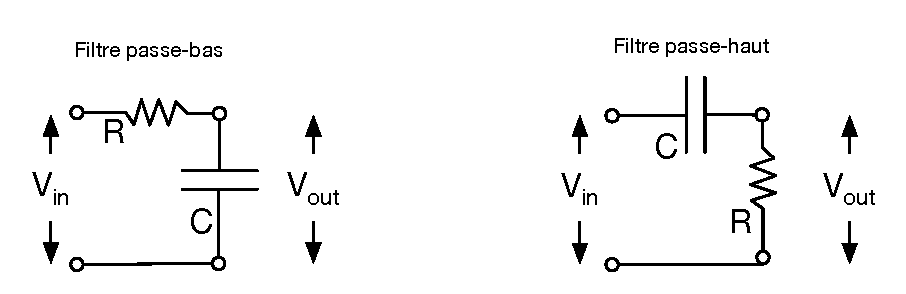
\includegraphics[width=15cm]{Labos-Complements/Lab07/FiltresPassifs_vDC.pdf} 
   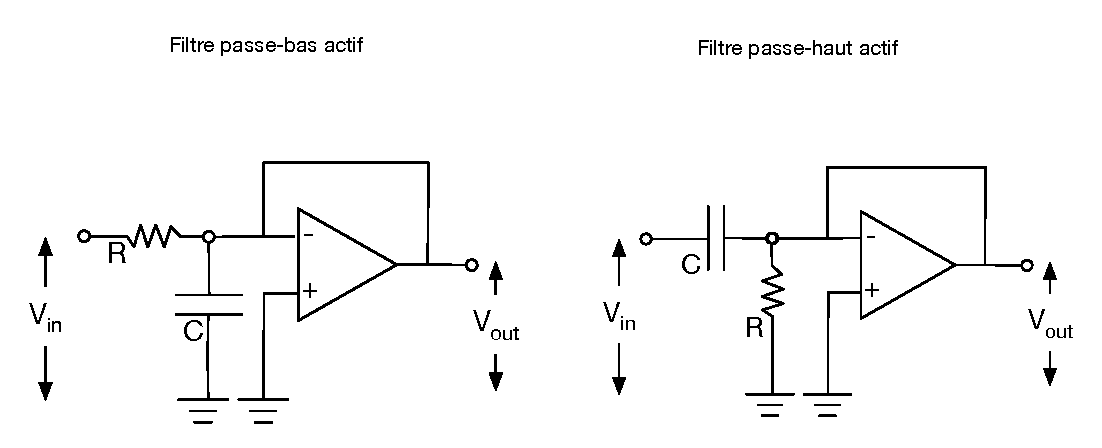
\includegraphics[width=15cm]{Labos-Complements/Lab07/FiltresActifsNonInverseurs_maisRCsur-_vDC.pdf} 
   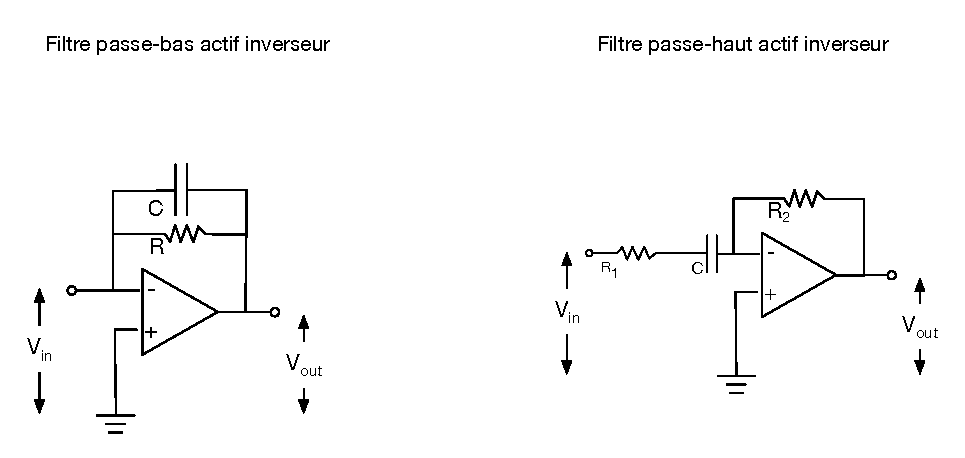
\includegraphics[width=15cm]{Labos-Complements/Lab07/FiltresActifsInverseurs_vDC.pdf} 
   \caption{Les filtres passifs (en haut) n'ont aucune source de puissance.  Il ne peuvent qu'atténuer des tensions, et leur impédance d'entrée et de sortie sont variables.  Au contraire, les filtres actifs ont une source de tension et apparaissent avec une impédance de sortie faible. Il y a plusieurs façons de faire des filtres, mais en voici deux sortes non-inverseurs (au centre) et inverseurs (en bas).}
   \label{fig:filtres}
\end{figure}
%Les ateliers se rapprochent d'un mode de travail expérimental plus professionnel, car vous devez vous-même préparer votre propre protocole avant d'arriver au laboratoire afin d'atteindre chaque sous-objectif énoncé ci-dessous. Ces sous-objectifs sont généralement accompagnés d'une figure de circuits, mais il y a toutefois progression vers une conception de plus en plus libre où vous devrez proposer vos propres design de circuits. Pour vous assister dans cette rédaction de protocole, les compléments en lecture préparatoire ci-dessus détaillent la théorie et les modèles pour comprendre le fonctionnement des circuits et les analyser expérimentalement. Concrètement dans votre cahier de recherche avec votre coéquipier.ère, écrivez des manipulations et des analyses à faire pour chaque sous-objectif afin de les mettre en commun en plus grand groupe lors de votre arrivée à la séance de laboratoire. 

\section{Déroulement de l’atelier}

Vous serez divisé en 6 groupes. Il y aura trois sources différentes (en 2 copies), pour trois situations différentes:
\begin{enumerate}
\item Une source "constante", qui varie lentement. Vous devez concevoir un filtre pour la stabiliser tout en gardant la tension lorsqu'une charge de 1 kOhms  est connectée.
\item Une source sinusoidale bruyante. Vous devez concevoir un filtre pour enlever le bruit hautes fréquences tout en gardant la tension lorsqu'une charge de 1 kOhms est connectée.
\item Une source analogique "constante" comme on trouve sur les Arduinos, de type Pulse Width Modulation. Vous devrez faire un filtre passe-bas qui fonctionnera, quelle que soit la résistance de charge utilisée, pour obtenir une tension proportionnelle constante.
\end{enumerate}

Chaque groupe choisira une source et travaillera à filtrer. Vous expliquerez ensuite faire une présentation orale éducative de 5~minutes pour le reste de la classe à la fin de la séance. 

Nous recommandons de commencer la séance en délibérant sur l'optimisation des manipulations expérimentales et des analyses proposées dans vos cahiers de recherche respectifs avec l'assistance du membre de l'équipe d'enseignement et il vous faudra ensuite répartir les tâches dans votre groupe. Des exemples de tâches possibles sont la planification et l'organisation, la conception, la simulation, la réalisation expérimentale, la mesure, l'analyse, la communication, etc. et il peut bien sûr y avoir de la redondance pour vérifier l'exactitude des résultats de mesure et d'analyse. Notez que la fin de la section \texttt{Matériel didactique} sur le site de cours propose différents choix de logiciels et d'applications pour vous assister dans les tâches de conception et de simulation.

La dernière activité de la séance sera de vous rendre sur le site Web du cours dans la section \texttt{Évaluations et résultats} pour l'atelier concerné et y évaluer vos pairs sur leur contribution respective au travail du groupe.
 
% \section{Les filtres: passifs et actifs}
%\begin{figure}[h!]
%\centering
%\begin{circuitikz} \draw
%(0,2) node[left]{$v_{\mathrm{g}}$} to[R=1~k$\Omega$,o-] (3,2) to[short,-o] (4,2) node[right]{$v_{\mathrm{out}}$}
%(3,2) to[C=1~$\mu$F] (3,0) node[ground]{}
%;\end{circuitikz}
%\caption{\label{sch-RC}\textbf{Sous-objectif}: observer et quantifier le délai temporel du signal en tension aux bornes des différents composants de ce même circuit RC série.}
%\end{figure}
%
%% a) Sur la plaquette de montage, réalisez le filtre RC de la figure~\ref{sch-RC} en utilisant le condensateur de précision ($\pm5$~\%).
%% \begin{figure}[h]
%% \centering
%% \begin{circuitikz} \draw
%% (0,2) node[left]{$v_{\mathrm{g}}$} to[R=1~k$\Omega$,o-] (3,2) to[short,-o] (4,2) node[right]{$v_{\mathrm{out}}$}
%% (3,2) to[C=1~$\mu$F] (3,0) node[ground]{}
%% ;\end{circuitikz}
%% \caption{\label{sch-RC}Circuit RC série.}
%% \end{figure}
%
%% b) Avec deux câbles coaxiaux et un «T», reliez la sortie du générateur de fonctions $v_{\mathrm{g}}$ à l'entrée du canal~1 de l'oscilloscope ainsi qu'à la plaquette de montage. À l'aide d'une sonde compensée (10X), reliez les bornes du condensateur au canal~2 de l'oscilloscope.
%
%% c) Générez un signal carré à 50~Hz allant de 0~V à 1~V. Sur l'écran de l'oscilloscope, faites afficher simultanément les deux signaux. En rapetissant les divisions de l'échelle horizontale, observez d'abord qualitativement comment varie la tension $v_{\mathrm{out}}$ et comparez avec le modèle présenté dans le complément \textit{Analyse temporelle}.
%
%% d) Mesurez le temps de montée (de 10~\% à 90~\%) et la constante de temps du circuit. Comparez avec les valeurs attendues.
%
%
%%\subsection{Partie 2 --- Mesures fréquentielles et diagrammes de Bode}
%
%\begin{figure}[h!]
%\centering
%\begin{circuitikz} \draw
%(0,2) node[left]{$V_{\mathrm{g}}$} to[R=270~$\Omega$,o-] (3,2) to[short] (3,2)
%(3,2) to[C=1~$\mu$F] (3,0) node[ground]{}
%;\end{circuitikz}
%\caption{\label{sch-RC2}\textbf{Sous-objectif} : démontrer que ce même circuit RC série agit en filtre passe-haut ou passe-bas en prenant les mesures appropriées pour construire les diagrammes de Bode du gain ET de la phase en fonction de la fréquence.}
%\end{figure}


\end{document}